\documentclass{article}

\usepackage{siunitx}
\usepackage{amsmath}
\usepackage{mathtools}
\usepackage{algorithm}
\usepackage{algpseudocode}
\usepackage{minted}
\usepackage{booktabs}
\usepackage{url}
\frenchspacing

\usemintedstyle{xcode}

\title{Project 1:\\Solution of a tridiagonal system of equations}
\author{Josh Bradt}
\date{February 12, 2016}

\begin{document}

\maketitle

\begin{abstract}
    In many cases, it is possible to rewrite a differential equation as a system of linear equations. We briefly describe this technique and then lay out the general solution to a system of linear equations using Gaussian elimination. Due to the inefficiency of this process, a more specialized algorithm is developed for solving systems involving tridiagonal matrices with constant diagonal elements. This code is tested and timed, and the results are compared to output from an LU-decomposition code.
\end{abstract}

\section{Introduction}

    Efficiently solving differential equations is essential to many problems in computational science. One particularly frequent class of differential equations are linear second-order differential equations, which can be written as
    \begin{equation}
        \frac{d^2 y}{dx^2} + k(x) y = f(x)  \label{eq:diffeq}
    \end{equation}
    for some source function $f(x)$ and a real function $k(x)$.

    One example of an equation of this form is found in classical electrostatics. There, the electric field of a point charge can be found using Poisson's equation:
    \begin{equation}
        \nabla^2 \Phi(\mathbf{r}) = -4\pi \rho(\mathbf{r})  \label{eq:poisson}
    \end{equation}
    where $\rho(\mathbf{r})$ is the charge distribution. Assuming spherical symmetry, this becomes a one-dimensional equation
    \begin{equation*}
        \frac{1}{r^2} \frac{d}{dr} \left( r^2 \frac{d\Phi}{dr} \right) = -4\pi\rho(r)
    \end{equation*}
    which can be written as
    \begin{equation*}
        \frac{d^2\phi}{dr^2} = -4\pi r \rho(r)
    \end{equation*}
    by letting $\Phi(r) = \phi(r) / r$. This is now a linear second-order differential equation of the form shown in (\ref{eq:diffeq}) where $k(r) = 0$ and $f(r) = -4\pi r \rho(r)$. To simplify things further, let $r \rightarrow x$ and $\phi \rightarrow u$, and then define $f(x) = -4\pi x \rho(x)$. Then our equation becomes
    \begin{equation*}
        -u''(x) = f(x).
    \end{equation*}
    Equations of this form can occasionally be solved analytically, but in general they must be solved using numerical methods.

\section{Numerical algorithm}

    To make the problem more concrete, we will be solving the equation
    \begin{equation}
        -u''(x) = f(x)  \label{eq:simple}
    \end{equation}
    on the domain $x \in [0, 1]$ with Dirichlet boundary conditions $u(0) = u(1) = 0$.

    \subsection{Transformation to linear equations}

        The second derivative can be found using the second-order finite difference relation
        \begin{equation}
            u''(x) \approx \frac{u(x+h) + u(x-h) - 2u(x)}{h^2} + O(h^2)  \label{eq:finite}
        \end{equation}
        for some small step size $h$. Plugging this relation into (\ref{eq:simple}) produces the equation
        \begin{equation}
            -\frac{u(x+h) + u(x-h) - 2u(x)}{h^2} = f(x).
        \end{equation}
        Next, we discretize the problem by creating a mesh of step size $h$ between the lower and upper boundaries. This is conceptually the same as representing the functions $u(x)$ and $f(x)$ as vectors $u_i$ and $f_i$. Thus, we can write
        \begin{equation}
            -\frac{u_{i+1} + u_{i-1} - 2u_i}{h^2} = f_i, \quad i = 1, \dots, n.
        \end{equation}
        Thinking of $u$ and $f$ as vectors, this can be interpreted as taking the $(i+1)$-th element of $u$, the $(i-1)$-th element of $u$, and so on. This leads to a natural interpretation of this equation in terms of a set of linear equations
        \begin{equation}
            \begin{pmatrix}
                 2 & -1 &        &        &    \\
                -1 &  2 & -1     &        &    \\
                   & -1 & \ddots & \ddots &    \\
                   &    & \ddots & \ddots & -1 \\
                   &    &        & -1     &  2
            \end{pmatrix}
            \begin{pmatrix}
                u_1 \\ u_2 \\ u_3 \\ \vdots \\ u_n
            \end{pmatrix}
            =
            \begin{pmatrix}
                w_1 \\ w_2 \\ w_3 \\ \vdots \\ w_n
            \end{pmatrix}
            \label{eq:oursystem}
        \end{equation}
        where $w_i \equiv h^2 f_i$, and all elements not shown in the matrix are taken to be zero. This is a \emph{tridiagonal} matrix, meaning it has elements only on the primary diagonal and on the diagonals above and below it.

        Rewriting the problem in this way turns the relatively difficult task of solving a differential equation into the well-studied task of solving a system of linear equations.

    \subsection{General Gaussian elimination}

        One of the most basic and well-known methods for solving linear equations is the method of Gaussian elimination. Solving a system of equations with this method consists of two steps: forward substitution and backward substitution.

        Starting with a general matrix
        \begin{equation*}
            \begin{pmatrix}
                a_{11} & a_{12} & a_{13} & a_{14} & w_1 \\
                a_{21} & a_{22} & a_{23} & a_{24} & w_2 \\
                a_{31} & a_{32} & a_{33} & a_{34} & w_3 \\
                a_{41} & a_{42} & a_{43} & a_{44} & w_4 \\
            \end{pmatrix}
        \end{equation*}
        with the solution vector $\mathbf{w}$ appended as the last column, the forward substitution step consists of adding multiples of each row to the rows below it until the matrix becomes upper-triangular. Thus, after one substitution, the original matrix above becomes
        \begin{equation*}
            \begin{pmatrix}
                a_{11} & a_{12}  & a_{13}  & a_{14}  & w_1 \\
                0      & a'_{22} & a'_{23} & a'_{24} & w'_2 \\
                0      & a'_{32} & a'_{33} & a'_{34} & w'_3 \\
                0      & a'_{42} & a'_{43} & a'_{44} & w'_4 \\
            \end{pmatrix}, \text{ where }
            \begin{dcases}
                a'_{ij} &= a_{ij} - \frac{a_{i1}}{a_{11}} a_{1j} \\
                w'_i    &= w_i - \frac{a_{i1}}{a_{11}} w_1
            \end{dcases}.
        \end{equation*}
        After a second substitution, it becomes
        \begin{equation*}
            \begin{pmatrix}
                a_{11} & a_{12}  & a_{13}   & a_{14}   & w_1   \\
                0      & a'_{22} & a'_{23}  & a'_{24}  & w'_2  \\
                0      & 0       & a''_{33} & a''_{34} & w''_3 \\
                0      & 0       & a''_{43} & a''_{44} & w''_4 \\
            \end{pmatrix}, \text{ where }
            \begin{dcases}
                a''_{ij} &= a'_{ij} - \frac{a'_{i2}}{a'_{22}} a'_{2j} \\
                w''_i    &= w'_i - \frac{a'_{i2}}{a'_{22}} w'_2
            \end{dcases}.
        \end{equation*}
        Finally, after a third substitution, we have
        \begin{equation*}
            \begin{pmatrix}
                a_{11} & a_{12}  & a_{13}   & a_{14}    & w_1   \\
                0      & a'_{22} & a'_{23}  & a'_{24}   & w'_2  \\
                0      & 0       & a''_{33} & a''_{34}  & w''_3 \\
                0      & 0       & 0        & a'''_{44} & w'''_4 \\
            \end{pmatrix}, \text{ where }
            \begin{dcases}
                a'''_{ij} &= a''_{ij} - \frac{a''_{i3}}{a''_{33}} a''_{3j} \\
                w'''_i    &= w''_i - \frac{a''_{i3}}{a''_{33}} w''_3
            \end{dcases}.
        \end{equation*}

        This pattern is described in the first part of the pseudocode in Algorithm~\ref{algo:gauselim}. In this formation, the variable $k$ represents the index of the row currently being subtracted from the other rows, and $i$ and $j$ represent the row and column being operated on. The multiplicative factor is computed once per row and stored in $C$ for efficiency.

        \begin{algorithm}
            \begin{algorithmic}
                \Require $a$ is an $N \times N$ array
                \Require $w$ is a length-$N$ vector
                \For {$k = 0, 1, \dots, N - 1$} \Comment{Forward substitution}
                    \For {$i = k + 1, k+2, \dots, N$}
                        \State $C \gets a_{ik} / a_{kk}$
                        \State $w_i \gets w_i - C w_k$
                        \For {$j = k, k+1, \dots, N$}
                            \State $a_{ij} \gets a_{ij} - C a_{kj}$
                        \EndFor
                    \EndFor
                \EndFor
                \For {$k = N, N-1, \dots, 1$} \Comment{Backward substitution}
                    \For {$i = k - 1, k - 2, \dots, 0$}
                        \State $C \gets a_{ik} / a_{kk}$
                        \State $w_i \gets w_i - C w_k$
                    \EndFor
                \EndFor
            \end{algorithmic}
            \caption{Gaussian elimination}
            \label{algo:gauselim}
        \end{algorithm}

        Once the forward-substitution step is complete, we proceed with backward substitution to fully diagonalize the matrix. This process only affects the solution vector $\mathbf{w}$. In the following steps, assume the $b_{ij}$ are the elements of the matrix after forward substitution is complete, and the $v_i$ are the elements of the solution vector after forward substitution.

        First, after one step of backward substitution, we have
        \begin{equation*}
            \begin{pmatrix}
                b_{11} & b_{12}  & b_{13}   & 0      & v'_1 \\
                0      & b_{22}  & b_{23}   & 0      & v'_2 \\
                0      & 0       & b_{33}   & 0      & v'_3 \\
                0      & 0       & 0        & b_{44} & v_4  \\
            \end{pmatrix}, \text{ where }
            v'_i = v_i - \frac{b_{i4}}{b_{44}} v_4 .
        \end{equation*}
        After a second step, this becomes
        \begin{equation*}
            \begin{pmatrix}
                b_{11} & b_{12}  & 0        & 0      & v''_1 \\
                0      & b_{22}  & 0        & 0      & v''_2 \\
                0      & 0       & b_{33}   & 0      & v'_3  \\
                0      & 0       & 0        & b_{44} & v_4   \\
            \end{pmatrix}, \text{ where }
            v''_i = v'_i - \frac{b_{i3}}{b_{33}} v'_3 .
        \end{equation*}
        And finally, the last step produces
        \begin{equation*}
            \begin{pmatrix}
                b_{11} & 0       & 0        & 0      & v'''_1 \\
                0      & b_{22}  & 0        & 0      & v''_2 \\
                0      & 0       & b_{33}   & 0      & v'_3  \\
                0      & 0       & 0        & b_{44} & v_4   \\
            \end{pmatrix}, \text{ where }
            v'''_i = v''_i - \frac{b_{i2}}{b_{22}} v''_3 .
        \end{equation*}
        At this point, the system of equations is clearly solved.

        This is clearly not the most computationally efficient algorithm for solving a system of equations. By inspecting the algorithm, we can see that the forward substitution step scales as $O(n^3)$, while the backward substitution step scales as $O(n^2)$. A more efficient method for solving our particular problem will be outlined in the next section.

    \subsection{A specialized algorithm}

        In Equation~\ref{eq:oursystem}, we showed that the equation that we're actually trying to solve consists of a tridiagonal matrix. This means that most of the elements are zeros, and the remaining elements only take one of two constant values. Therefore, if we use the general algorithm described in the previous section, it will mostly be wasting time repeating the same calculations. Additionally, it's a waste of memory to represent the equation using a dense matrix, and it may become impossible to do so as the step size gets smaller.

        The matrix can be represented more efficiently if we look carefully at its elements. The upper and lower diagonal elements are all equal to $-1$, and the Gaussian elimination process will not change any of these elements since the upper diagonal has all zeros above it, and the lower diagonal will always be set to 0 by the forward substitution step. Therefore, we can represent these two diagonals with two scalar constants. The main diagonal's elements do change, so we represent this as a one-dimensional array. This reduces the memory used for storing the matrix from $O(n^2)$ to roughly $O(n)$.

        Reducing the number of elements stored also immediately reduces the number of operations to be performed. Algorithm~\ref{algo:gausspecial} shows that by ignoring the zero elements of the array and only iterating over the elements of the main diagonal, the number of floating point operations is reduced from being cubic in $n$ to being linear (or, more specifically, $O(8n)$). An implementation of this algorithm in C++ is included in Appendix~\ref{sec:cimpl}.

        \begin{algorithm}[t]
            \begin{algorithmic}
                \Require {$a, c$ are constants equal to the upper and lower diagonals}
                \Require {$b$ is a length-$N$ vector representing the diagonal elements}
                \For {$i = 1, 2, \dots, N$} \Comment {Forward substitution}
                    \State $M \gets a / b_{i-1}$
                    \State $b_i \gets b_i - Mc$
                    \State $w_i \gets w_i - Mw_{i-1}$
                \EndFor
                \For {$i = N-1, N-2, \dots, 0$} \Comment {Backward substitution}
                    \State $w_i \gets w_i - \frac{c}{b_{i+1}} w_{i+1}$
                \EndFor
            \end{algorithmic}
            \caption{A specialized Gaussian solver}
            \label{algo:gausspecial}
        \end{algorithm}

    \section{Results}

        The algorithm described above was run for matrices with $n$ equal to 10, 100, and 1000 to   solve the differential equation for the source function
        \begin{equation}
            f(x) = 100 e^{-10x}.
        \end{equation}
        The differential equation has an analytic solution
        \begin{equation}
            u(x) = 1 - (1 - e^{-10}) x - e^{-10x}
        \end{equation}
        for this source function, which provides a convenient way to check that our algorithm is correct.

        \subsection{Convergence}

            The calculated results are compared to the analytic result in Fig.~\ref{fig:convergence}.

            \begin{figure}
                \centering
                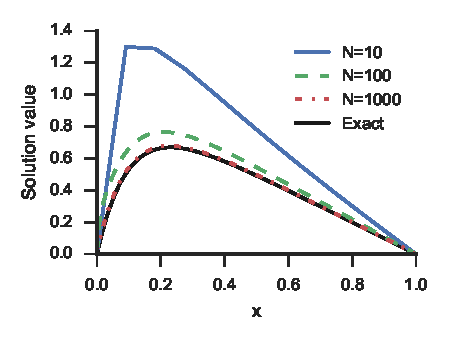
\includegraphics{convergence.pdf}
                \caption{Convergence of the algorithm for varying values of $n$. The solid black line shows the correct, analytic solution. The results are converging on this solution as $n$ increases.}
                \label{fig:convergence}
            \end{figure}

            The relative error in the calculated result can be represented on a log scale as
            \begin{equation}
                \epsilon_i = \log_{10}\left(\left| \frac{v_i - u_i}{u_i} \right| \right)
            \end{equation}
            where $v_i$ is the calculated result and $u_i$ is the analytic result. This value is plotted for $n=10$, $n=100$, and $n=1000$ in Fig.~\ref{fig:relerror}. The relative error decreases for increasing values of $n$, but the precision is ultimately limited by the precision of floating point arithmetic. This is apparent in Table~\ref{tab:error}, which shows the maximum relative error for $n$ up to $n=10^5$.

            \begin{table}
                \centering
                \begin{tabular}{cc}
                    \toprule
                    $n$    & $\epsilon$ \\
                    \midrule
                    $10^1$ & 0.1953 \\
                    $10^2$ & 0.2937 \\
                    $10^3$ & 0.3034 \\
                    $10^4$ & 0.3010 \\
                    $10^5$ & 0.3010 \\
                    \bottomrule
                \end{tabular}
                \caption{Maximum relative error for increasing values of $n$. The benefit of increasing $n$ eventually diminishes due to floating point error.}
                \label{tab:error}
            \end{table}

            \begin{figure}
                \centering
                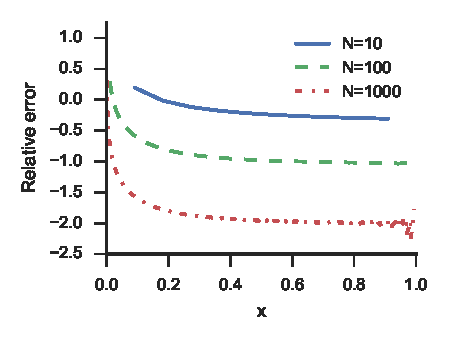
\includegraphics{relerror.pdf}
                \caption{Relative error $\epsilon$ in the calculated results. The error decreases with larger $n$, but eventually the result is limited by numerical precision.}
                \label{fig:relerror}
            \end{figure}

        \subsection{Performance}

            To assess the accuracy of the $O(n)$ performance estimate given above, the runtime of the code was measured for several values of $n$. The runtime was measured using the functionality built into the C++ standard library \texttt{chrono} header (available since C++11). For comparison, a comparable code was constructed using the LU decomposition and linear equation solver functions built into the Armadillo linear algebra library\footnote{\url{http://arma.sourceforge.net}} and timed for the same values of $n$. The timing results are listed in Table~\ref{tab:timing} and plotted in Fig.~\ref{fig:timing}, and the convergence of the two codes to the correct answer is compared in Fig.~\ref{fig:convcomp}.

            For the timing tests, the codes were compiled on a Mac OS X 10.11.3--based system with an Intel Core i7 processor running at \SI{2.3}{GHz}. The compiler was the default Apple-provided Clang version 7.0.2, and the optimization level used was \texttt{-O3}.

            \begin{table}
                \centering
                \begin{tabular}{S[table-format=6]
                                S[table-format=1.4e+1]
                                S[table-format=1.4e+1]}
                    \toprule
                    {$N$} & {Gaussian solver time [s]} & {Armadillo LU time [s]} \\
                    \midrule
                        10 & 4.4121e-07 & 2.8043e-06 \\
                       100 & 3.0373e-06 & 6.4414e-04 \\
                      1000 & 2.8477e-05 & 4.0147e-02 \\
                     10000 & 2.7965e-04 &   {-}         \\
                    100000 & 2.8545e-03 &   {-}        \\
                    \bottomrule
                \end{tabular}
                \caption{Comparison of time taken by the two codes. The Armadillo-based LU decomposition code did not finish for the largest two values of N.}
                \label{tab:timing}
            \end{table}

            \begin{figure}[p]
                \centering
                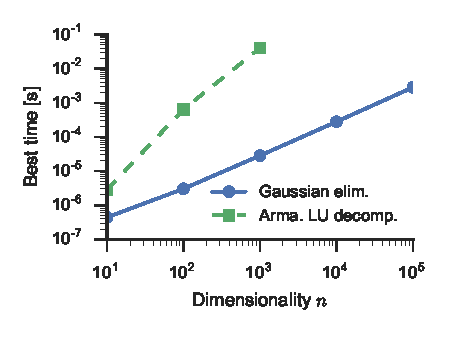
\includegraphics{times.pdf}
                \caption{Timing comparison of Armadillo LU decomposition code versus the code presented in this paper.}
                \label{fig:timing}
            \end{figure}

            \begin{figure}[p]
                \centering
                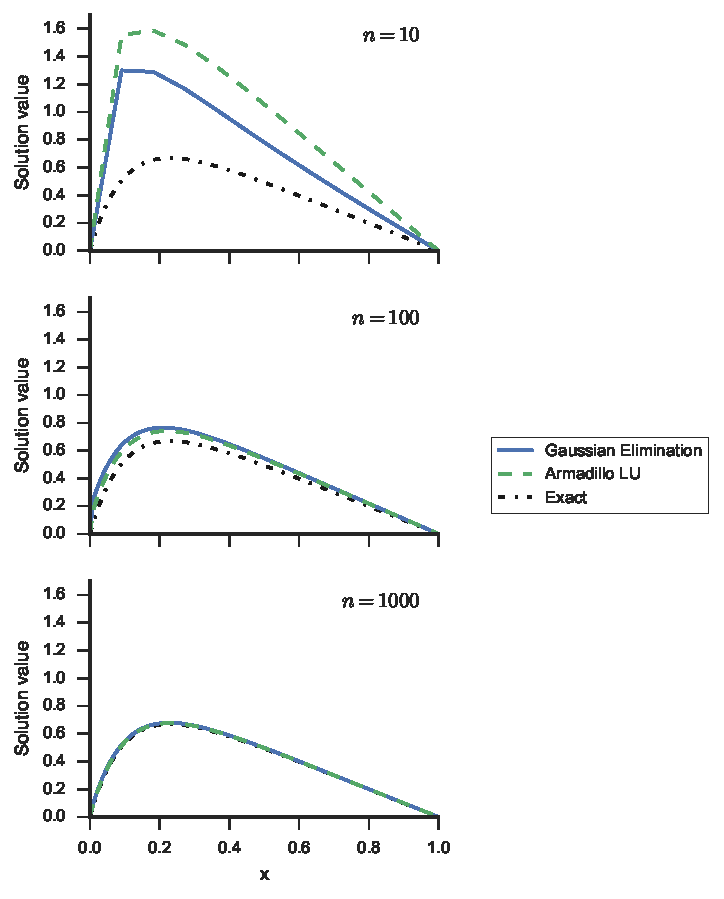
\includegraphics{conv_vs_arma.pdf}
                \caption{A comparison of the convergence of the Gaussian elimination code presented in this paper to the convergence of the LU decomposition code.}
                \label{fig:convcomp}
            \end{figure}

\section{Conclusion}

    Although the generic Gaussian elimination algorithm is quite inefficient with $O(n^3)$ performance, the specialized version of it presented here for tridiagonal matrices performs significantly better, even when compared to LU decomposition codes. This is, however, almost entirely due to the symmetries of the tridiagonal matrix which we exploited when simplifying the general algorithm. Although this makes these results inapplicable to general situations, it does illustrate that it can sometimes be very beneficial to tailor a solution to a particular problem.

\pagebreak

\appendix

\section{C++ implementation of the specialized Gaussian solver}
\label{sec:cimpl}

    \begin{minted}[gobble=8]{C++}
        #include <vector>
        #include <functional>  // Requires C++11

        inline double findStepSize(const double lb, const double ub,
                                   const unsigned long numPts)
        {
            return (ub - lb) / (numPts + 1);
        }

        std::vector<double>
        solveEquation(const std::function<double(double)>& f,
                      const unsigned long numPts)
        {
            // f is the source function from the right-hand side of the equation
            // numPts determines the step size and dimensions of the matrix

            const double a = -1;  // Upper diagonal
            const double c = -1;  // Lower diagonal
            const double stepSize = findStepSize(0, 1, numPts);
            std::vector<double> bs (numPts + 2, 2);  // Main diagonal
            std::vector<double> ws (numPts + 2, 0);  // Solution

            // Initialize solution with f
            for (size_t i = 1; i < numPts + 1; i++) {
                ws.at(i) = f(i*stepSize) * stepSize * stepSize;
            }

            // Forward substitution
            for (size_t i = 1; i < numPts + 1; i++) {
                double factor = a / bs.at(i-1);
                bs.at(i) -= factor * c;
                ws.at(i) -= factor * ws.at(i-1);
            }

            // Backward substitution
            for (size_t i = numPts - 1; i > 0; i--) {
                ws.at(i) -= c / bs.at(i+1) * ws.at(i+1);
            }

            return ws;
        }
    \end{minted}


\end{document}
